\documentclass[letterpaper]{article} %DO NOT CHANGE THIS
\usepackage{aaai19}  %Required
\usepackage[ruled,vlined,linesnumbered]{algorithm2e}
\usepackage{times}
\usepackage{helvet}
\usepackage{color}
\usepackage{graphicx}
\usepackage{courier}
\usepackage{amsthm}
\usepackage{amsmath}
\usepackage{url}
\usepackage{algorithmic}
\usepackage{subcaption}
\usepackage{todonotes}
\usepackage{multirow}
\usepackage{xcolor}

\usepackage{tabu}
\usepackage{array}
\usepackage{natbib}
\usepackage{arydshln}

\newtheorem{example}{Example}
\newtheorem{lemma}{Lemma}
\newtheorem{theorem}{Theorem}


\newcommand\note[1]{\textcolor{red}{#1}}
\newcommand\commentout[1]{}

\theoremstyle{definition}
\newtheorem{definition}{Definition}[section]


\frenchspacing


\newcolumntype{?}{!{\vrule width 1pt}}

\newcommand\gNote[1]{\todo[inline, author=Guy, color=pink]{#1}}



\setlength{\belowcaptionskip}{-10pt}



\setcounter{secnumdepth}{2}

\begin{document}

\title{Improved Knowledge Modeling and Its Use for Signaling\\ in Multi-Agent Planning with Partial Observability}

\author{
Shashank Shekhar\\
Department of Computer Science\\
Ben Gurion University\\
shekhar@cs.bgu.ac.il\\
\And
Ronen I. Brafman\\
Department of Computer Science\\
Ben Gurion University\\
brafman@cs.bgu.ac.il
\And
Guy Shani\\
Information and Software Systems Eng.\\
Ben Gurion University\\
shanigu@bgu.ac.il
}

\maketitle

\begin{abstract}
Collaborative Multi-Agent Planning (MAP)
problems with uncertainty and partial observability
are often modeled as Dec-POMDPs. Yet,
in deterministic domains, {\em Qualitative}
Dec-POMDPs can scale up to much larger problem sizes.
The best current QDec solver
(QDec-FP)
reduces MAP problems to multiple single-agent problems.
In this paper we describe a planner that uses richer information about agents' knowledge to improve upon QDec-FP.
With this change, the planner not only scales up to larger problems with more objects, but it can also support
{\em signaling}, where agents signal information to each other by changing the state of the world.
\end{abstract}

\section{Introduction}

In many real-world problems, agents collaborate to achieve joint goals. For example, disaster response teams typically consist of agents that have multiple tasks to perform,
some of which require the cooperation of several agents.
In such domains, agents may have partial information, where they can sense only their immediate surroundings.
As agents are often located in different positions and may possess different sensing abilities, their runtime information states differ.  While this can be overcome using communication, the communication infrastructure can be damaged, or communication may be costly and should be reasoned about explicitly.

In this setting, it is common to compute a policy for all agents %jointly
using a central engine.
This policy is executed by the agents in a decentralized manner, and agent communication is performed through explicit actions. Decentralized POMDPs (Dec-POMDPs) offer a rich model for capturing such multi-agent problems~\citep{Bernstein02,OliehoekA16}, but Dec-POMDP solvers have difficulty scaling up.  Qualitative Dec-POMDPs (QDecs) were introduced as an alternative model, replacing the
probability distributions over possible states with qualitative sets of states~\citep{BrafmanSZ13}.
QDecs can also be viewed as the multi-agent extension of the well known Contingent Planning model~\citep{hoffmann2005contingent}.
At least for deterministic problems, where partial observability plays the key role, QDec algorithms scale much better than Dec-POMDP algorithms.
This was demonstrated clearly by the IMAP solver~\citep{IMAP}, which was later improved
by the QDec-FP planner~\citep{ShekharBS19}.

QDec-FP solves an abstract and simplified centralized problem which they call the {\em team problem.}
It is the single-agent problem, where the single agent is the entire team. This problem can be solved by a single-agent contingent solver.
However, its solution
is not necessarily executable by the agents. It may require that agent $\varphi_j$ act differently based on the value of some proposition $p$ observed by agent $\varphi_i$, even if $\varphi_j$ cannot observe $p$.
To fix this, a second set of planning problems is solved, in which each agent attempts to generate a plan that emulates its behavior in the solution to the team problem (which may require it to perform additional sensing, for example).
If this  second stage of QDec-FP is successful, we get a correct, executable solution. If it is not, the planner attempts to generate a new team plan.

In this paper we describe a new algorithm, QDec-FPS, which uses enhanced reasoning about the  knowledge of {\em individual} agents in the team problem.
Reasoning about individual agents' knowledge
during team plan execution has two important advantages: First, it will lead to the generation of more informed team plans that are easier to extend to true solutions, because the team planner adds an action only if the agent that executes it knows that its preconditions hold.
Second, it allows us to model, within the team plan, the process of explicit and implicit communication, which we refer to here as {\em signaling.}



Signaling refers to cases where agent $\varphi_i$ can sense $p$ but agent $\varphi_j$ cannot.
$\varphi_i$  communicates this information to $\varphi_j$ by setting the value of some variable $q$ that agent $\varphi_j$ can sense, to be correlated with the value of $p$. For example,  $\varphi_j$ cannot sense whether a door is open, but it can sense whether the light is on, while agent $\varphi_i$ can sense both. If $\varphi_i$ can also turn the light on and off, it can signal the door state to $\varphi_j$ by turning on the light if and only if the door is open.



Technically, signaling consists of the following steps: $(1)$ Agent $\varphi_i$ senses $p$. $(2)$ Agent $\varphi_i$ sets the value of $q$ to the value of $p$. $(3)$ Agent $\varphi_j$ senses $q$.
To be sound, this behavior must be consistent between the two execution branches that follow the sensing of $p$: if $p$ is \emph{true}, we must ensure $q$ is \emph{true}.
If $p$ is \emph{false}, we must ensure $q$ is \emph{false}.
Note that, to support signaling, the planner must model the knowledge of each agent within the team plan. For otherwise, the planner has no reason to insert signals into the plan because signaling does not enhance the knowledge of the team. Moreover, some problems cannot be solved without signaling.













\section{Background}


The flat-space QDec model is defined as follows:
\begin{definition} A qualitative decentralized partially observable Markov decision process
(QDec) is a tuple ${\cal Q} = \langle  I, S, b_0,\{A_i | i\in I\}, \delta, \{\Omega_i\}, O, G\rangle$
where
\begin{itemize}
\item $I$ is a finite set of agents indexed $1,...,m$. We often refer to the $i^{th}$ agent as $\varphi_i$.

\item $S$ is a finite set of states.

\item$b_0 \subset S$ is the set of states initially possible.

\item  $A_i$ is a finite set of actions available to agent $\varphi_i$,
and $\vec{A} = \otimes_{i \in I} A_i$ is the set of joint actions,
where
$\vec{a} = {a_1,...,a_m}$ denotes a particular joint action.

\item $\delta: S \times \vec{A} \rightarrow 2^S$ is a non-deterministic Markovian transition function. $\delta(s, \vec{a})
$ denotes the set of states the can be reached when taking joint action $\vec{a}$ in state $s$.

\item $\Omega_i$ is a finite set of observations available to agent $\varphi_i$ and
$\vec{\Omega} = \otimes_{i \in I} \Omega_i$ is the set of joint
observation, where $\vec{o} = {o_1,...,o_m}$ denotes a particular joint
observation.

\item $\omega : \vec{A} \times S \rightarrow 2^{\vec{\Omega}}$ is a {\em non-deterministic\/} observation function. $\omega(\vec{a}, s)$
denotes the set of possible joint observations $\vec{o}$ given that
joint action $\vec{a}$ was taken and led to outcome state $s$. Here $s \in S,\, \vec{a}
\in \vec{A},\, \vec{o} \in \vec{\Omega}$.

\item $G \subset S$ is a set of goal states.

\end{itemize}
\label{11_def:DEC-POMDP}
\end{definition}

We focus on {\em deterministic outcomes} and {\em deterministic observations}. In such cases a successful solution is acyclic, and there is no need to bound the number of steps.
We assume a shared initial belief, like most Dec-POMDP models.

A factored QDec representation is specified as follows: $\langle I,P,\{A_i | i\in I\},\mathit{Pre},\mathit{Eff},\mathit{Obs},b_0,G\rangle$. $I$ is a set of agents, $P$ is a set of primitive propositions, $\vec{A}$ is a vector of individual action sets,  $\mathit{Pre, Obs,} \text{ and } \mathit{Eff}$ are the precondition, observation, and effects functions,
$b_0$ is the initial state formula, and $G$ is a set (conjunction) of goal propositions.


The state space, $S$, consists of all truth assignments to $P$. Each state can be viewed as a set of literals. Initial states are those that satisfy the initial state formula. Goal states are those that satisfy the goal conjunction.
The transition function,
$\delta$, is defined using  $\mathit{Pre}$ and  $\mathit{Eff}$ as follows:
The precondition function $\mathit{Pre}$ maps each individual action $a_i\in A_i$ to its set of preconditions, i.e., a set of literals that must
hold whenever agent $\varphi_i$ executes $a_i$. Preconditions are local, i.e., defined over $a_i$ rather than $\vec{a}$, because each agent must ensure that the relevant preconditions hold prior to executing its part of the joint action. We extend $\mathit{Pre}$ to be defined over joint actions $\{\vec{a}=\langle a_1,..,a_m\rangle : a_i \in A_i\}$ (where $m=|I|$):
$\mathit{Pre}(\langle a_1,..,a_m\rangle) = \cup_i \mathit{Pre}(a_i)$.

Following~\citet{IMAP}, we employ a more structured definition of joint actions.
We assume that single-agent actions are not executed concurrently unless specified explicitly using
{\em collaborative actions.} Collaborative actions have the same form as single-agent actions, except that they have multiple agent parameters.
Thus, an agent may have a single-agent {\em move} action, as well as participate in a
collaborative, two-agent action, {\em joint-lift}, for lifting a table.
Later, the plan can be made more
compact in post-processing, e.g., using the technique of~\citet{CJR14}. For a deeper discussion of the definition of joint actions, see, e.g.,~\citep{ShekharB18,ShekharB20}.

For every joint action $\vec{a}$ and agent $\varphi_i$, $\mathit{Obs}(\vec{a},i)=\{p_1,\ldots,p_k\}$, where $p_1,...,p_k$ are the propositions whose value agent $\varphi$ observes after the joint execution of $\vec{a}$. The observation is private, i.e., each agent may observe different aspects of the world. We assume that the observed value is correct and corresponds to the post-action variable value.

We also assume that actions either sense or change the state of the world. Sensing actions do not affect the world state --  their effect list is empty.  Non-sensing actions provide
no information -- their observation list is empty. This is not a limiting assumption, as every action can be separated into a non-observation and a sensing action by adding suitable propositions forcing the two to appear consecutively in every plan. Finally, we assume every agent has a $noop$ action, with $\mathit{Pre}(noop)=\mathit{Eff}(noop) =\mathit{Obs}(noop)= \emptyset$.


Another important concept in multi-agent planning is the notion of {\em public} and {\em private} actions and propositions~\citep{brafman2008one}.
A proposition that appears in the action descriptions of multiple agents is called {\em public}. Also, all goal propositions are public.
An action is a {\em public action} if its precondition or effect contain a public proposition.
A proposition that appears only in the actions of agent $\varphi_i$ is called {\em private} to  $\varphi_i$. An action whose preconditions and effects contain only private propositions is a {\em private action}.




The local plan of an agent $\varphi$ is represented by a \emph{policy tree} $\tau_i$.  Each node is labeled with an action, and edges that follow a sensing action are labeled by an observation.  The agent performs the action at the root and continues to the subtree labeled with the observation it obtained.

Given policy tree $\tau_i$ for agent $\varphi_i$, and an $o_i$, $\tau_{i_{o_i}}$ denotes the child subtree of the root of $\tau_i$ that is reached via a branch labeled by $o_i$.
Let $\vec{\tau} = \langle  \tau_1, \tau_2, \cdots, \tau_m \rangle$ be a vector of policy trees, one per agent,
also called a {\em joint policy}.
We denote the joint action at the root of $\vec{\tau}$ by $\vec{a}_{\vec{\tau}}$, and for an observation vector
$\vec{o}=o_1,\ldots, o_m$, containing each agent's observation, we define $\vec{\tau}_{\vec{o}}= \langle  \tau_{1_{o_1}},\ldots, \tau_{m_{o_m}}\rangle$.

As actions may have preconditions, a joint policy tree is executable only if the preconditions of each action hold prior to its execution. To check this, we can maintain the set of states possible at each node during the execution of the joint policy, called the
\emph{belief state}. Initially, it consists of all possible initial states, denoted $b_0$.
After an agent with belief state $b_i$ executes the first action of its current policy $\tau_i$, $a_{\tau_i}$, and observes ${o_i}$, its new belief state is
$tr(b_i,o_i,{a}_{\tau_i}) = \{a_{\tau_i}(s) | s\in b_i, a_{\tau_i}(s)\models o_i\}$.
Similarly the {\em team} belief state is
initially $b_0$. After executing the initial action of joint-policy $\tau$ given belief state $b$, it is updated to
$tr(b,\bar{o},\bar{a}_{\tau}) = \{\bar{a}_{\tau}(s) | s\in b, \bar{a}_{\tau}(s)\models \bar{o}\}$.
Naturally,
online, each agent may have less information than the combined team, as it does not know what other agents observed, and it cannot distinguish between all branches of the {\em joint}-policy. We denote by $\vec{b}$ the set of agent-specific beliefs.

To follow policy $\vec{\tau}$, we first consider the action $\vec{a}_{\vec{\tau}}$ given the current belief state $b$. It must be the case that
$b \models pre(a_{\tau})$. In that case, we say that  $\vec{a}_{\vec{\tau}}$ is {\em executable} in $b$.
A  joint policy  $\vec{\tau}$ is {\em executable} in belief  $b$ if (1) $\vec{a}_{\vec{\tau}}$ is executable in $\vec{b}$;  (2) if $a_{\tau_i}$ is  part of a collaborative action and $j$ is another agent participating in that collaborative action, then $a_{\tau_j}$ contains $j$'s part of that action;
(3) For every possible joint observation $\vec{o}$,    $\vec{\tau}_{\vec{o}}$ is executable given $tr(b,\vec{o},\vec{a}_{\vec{\tau}})$.

A joint policy is called a {\em solution} if it is executable in $b_0$, and the belief state in all leaf nodes in the tree satisfies $G$.
Note that unlike Dec-POMDPs, for QDecs there is no obvious notion of optimal policy, or optimization criterion, although one could strive to find trees with smaller depth, or trees that minimize the maximal branch cost.

\begin{figure}[t]
\centering
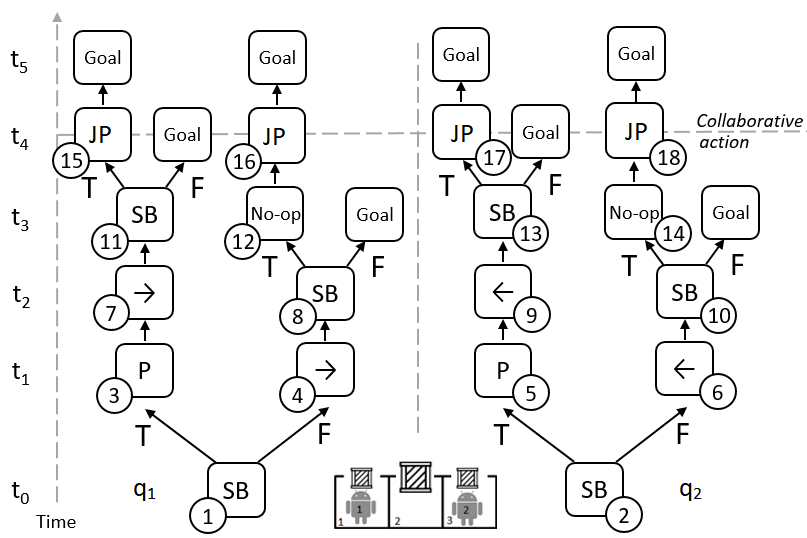
\includegraphics[width=3.3in]{LocalTrees.png}
\caption{\emph{SB} denotes sensing box, arrows denote motion, {\em P} denotes push,
and \emph{JP} denotes joint-push.
}
\label{fig:LocalTrees}
\end{figure}


\begin{example}
\label{ex:BoxPushing}
We have a 1D grid of size 3, with cells marked 1-3. The two agents $\varphi_1$ and $\varphi_2$ start in cells 1 and 3. Each cell may contain a box that needs to be pushed upwards. The left and right boxes are light and can be pushed
by a single agent. The middle box is heavy and can
be pushed by two agents acting together. Thus,
$P=\{\mathit{AgentAt}_{i,pos},\mathit{BoxAt}_{j,pos},\mathit{Heavy}_{j}\}$ where $pos \in \{1,2,3\}$ is a grid position, $i \in \{\varphi_1,\varphi_2\}$, and $j \in \{1,2,3\}$ is a box index. In the initial state each box may be in or out of the grid --- $b_0=\mathit{AgentAt}_{\varphi_1,1} \wedge \mathit{AgentAt}_{\varphi_2,3} \bigwedge_{j=1,2,3} (BoxAt_{j,j} \vee \neg BoxAt_{j,j})$. There are therefore 8 possible initial states.

Agents can move left and right, push a light box up, or jointly push a heavy box up. There are no preconditions for moving left and right. The agent must be
in the same cell as the box to push it.
There also actions for sensing for boxes --- $\mathit{SenseBox_{\varphi,j}}$, with precondition $\mathit{Pre(SenseBox_{\varphi,j})}=AgentAt_{\varphi,j}$, no effects, and $\mathit{Obs(SenseBox_{\varphi,j})}=BoxAt_{j,j}$.
The goal is to move all boxes out of the grid, i.e., $\bigwedge_j \neg BoxAt_{j,j}$.

Figure~\ref{fig:LocalTrees} illustrates this domain and a possible solution.
\end{example}

In what follows  {\em projected sub-tree} denotes a tree  obtained from the original policy tree by removing some nodes. When a node $n$ labeled by a non-sensing action is removed, the parent of $n$ becomes the parent of the child of $n$. A node $n$ labeled by a sensing action can only be removed if the two child subtrees of $n$ are identical. In that case, the parent of $n$ becomes the parent of one of the identical subtrees.





\section{The QDec-FP Algorithm}

QDec-FP~\citep{ShekharBS19} operates in three stages. (1) Generate a team solution. (2) Extend the projection of the team solution for each single agent. (3) Align the single agent plan trees.
In the first step, the MA problem is transformed into a single-agent problem by treating all actions as if executed by the same meta-agent. This meta-agent can apply any agent's action and and it is aware at each stage of the results of all sensing actions. We denote the resulting team plan as $\tau_{team}$.

In the second step, from $\tau_{team}$, QDec-FP generates for each agent $\varphi_i$ a projection $\tau_{\varphi_i}$. To obtain $\tau_{\varphi_i}$ we first remove from $\tau_{team}$ all non-sensing actions except those executed by agent $\varphi_i$. Next, we remove all private actions of all agents, leaving only nodes labeled by public actions.
Furthermore, for each action $a$ in $\tau_{\varphi_i}$, we remove all its public preconditions, as they are guaranteed to be supplied by some public action in $\tau_{team}$.
Finally we remove redundant sensing actions --- observations that do not influence how $\varphi_i$ acts. These are sensing actions where both subtrees below the observation are identical, from the perspective of agent $\varphi_i$.

An example of a team solution, its projection, and the compacted projection is given in Figure~\ref{fig:projected}.  Figure~\ref{fig:projected}A shows the team solution, containing both private and public actions of the %two
agents. The team plan assumes shared knowledge.
For example,
in the left branch, only agent $\varphi_1$ senses for the existence of the heavy box, but then both agents jointly push it. Figure~\ref{fig:projected}B shows the projected tree of $\varphi_1$. Private actions of both agents were removed, but sensing actions of both agents remain,
as no sensing action is redundant. Figure~\ref{fig:projected}C shows the projected tree of $\varphi_2$. The public {\em push} action executed by $\varphi_1$ in the team plan was removed. And since $\varphi_2$ operates identically in both subtrees of the team plan, we remove the sensing action at the root of the team plan.

\begin{figure*}[h!]
\centering
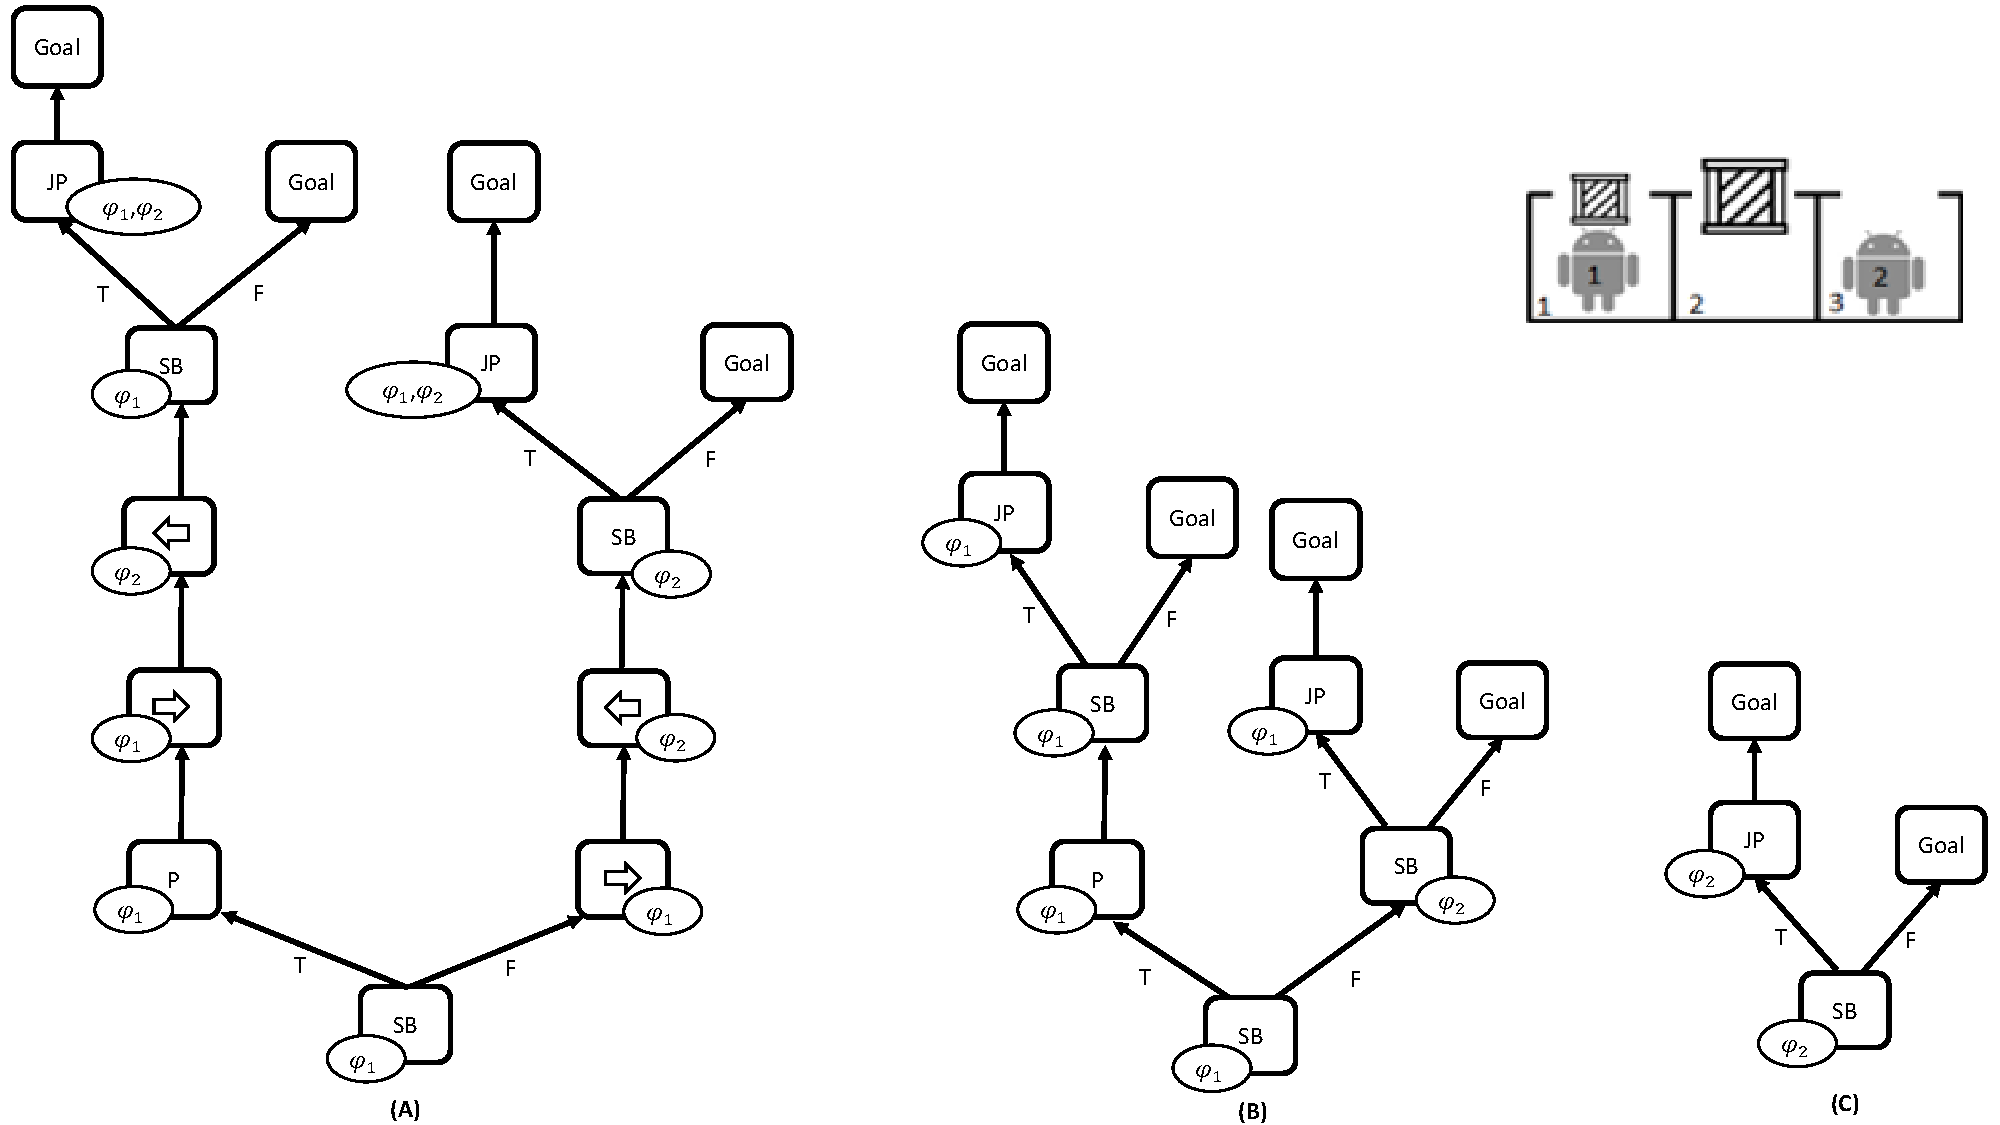
\includegraphics[width=0.8\textwidth, height=2.6in]{main-projection.pdf}
\caption{(A) Team plan tree $\tau_{team}$ for a problem with two agents, a light box and a heavy box that need to be pushed out.
(B) The projection of $\tau_{team}$ to $\varphi_1$.
(C) A compacted projection for $\varphi_2$.
}
\label{fig:projected}
\end{figure*}

The projected tree is typically not executable by the agent. It contains sensing actions that are executed by other agents, and some actions require additional preconditions, due to the removal of private actions.
Next, QDec-FP solves a single-agent contingent planning problem for each agent $\varphi_i$ that requires $\varphi_i$ to make $\tau_{\varphi_i}$ executable by adding sensing actions and private actions.
QDec-FP does not add public actions, as they could interfere with the policies of the other agents by, e.g., consuming a precondition that is needed.

If some $\tau_{\varphi_i}$ is not solvable, QDec-FP backtracks and seeks a new team solution.
If all $\tau_{\varphi_i}$ are solvable, we know that there is a solution, and all that remains is to align the different policies to ensure that agent actions are executed in the right order -- as reflected by the team policy. This is done by inserting $noop$ actions to postpone actions as need to be.

To implement QDec-FP,
one needs a single-agent off-line contingent planner.
QDec-FP uses CPOR~\citep{CPOR}, which generates a policy tree by repeatedly calling the online contingent planner SDR~\citep{SDR}. SDR generates a single execution branch that corresponds to the true initial state. CPOR
simply calls it multiple times with different "true" initial states.

While CPOR is the most scalable offline contingent planner currently, it has a major weakness: it does not backtrack.
To overcome this, QDec-FP introduced a backtracking mechanism on top of CPOR. It modifies the planning problem with an additional, sound, constraint, that invalidates
previous solutions.
However, this limits the number of backtracks that are practically possible.



\section{The QDec-FPS Planner}
QDec-FPS
has the
same high-level structure as QDec-FP, but modifies the way the team problem is solved, and adds a %pre-processing
mechanism for generating macros that enable signaling.


\subsection{Agent Specific Knowledge}


QDec-FP uses, through the CPOR planner, the SDR translation from contingent planning to classical planning. This translation maintains, for each proposition $p$, two propositions: $Kp$ and $K\neg p$, denoting knowing that $p$ is true or false, respectively.
SDR then transforms each precondition $p$ of an action to $Kp$.
The translation ensures that $Kp$ holds in a belief state only if $p$ holds in all possible worlds.
This is done by reasoning about all the specific possible worlds explicitly.

The state description in the classical translation contains the current state of the world given every possible initial state, in the form of $Kp|s$, where $p$ is a proposition, and $s$ is a possible state. It also contains actions that allow deducing new knowledge facts, called {\em merge} and {\em refutation} actions~\citep{PalaciosG09}. Thus, the agent can also obtain $Kp$ if for every currently possible state $s$, $Kp|s$ holds.



Because QDec-FP solves the team problem as a single-agent planning problem, the planner treats all agents as part of a single centralized agent, and the knowledge of this agent reflects the combined knowledge of all agents. Thus, when one agent observes that $p$ holds, other agents can use this knowledge, without observing the value of $p$ themselves. This is inconsistent with the real plan tree, where each agent must independently ensure that $p$ holds, before executing an action that requires $p$ as precondition.

QDec-FPS changes SDR's translation to be agent aware.
The $Kp$ propositions used to capture combined knowledge
are replaced by propositions of the form $K_{\varphi}p$, denoting that agent $\varphi$ knows that $p$ holds. The precondition $p$ of an action executed by agent $\varphi$ is replaced with  $K_{\varphi}p$. The effect of a sensing action executed by $\varphi$ is that only the sensing agent $\varphi$ knows the value of $p$, i.e., either $K_{\varphi}p$ or $K_{\varphi}\neg p$.
Similarly, merge and refutation actions now provide  agent-specific inference. The effect of a non-sensing action is still known to all agents (as agents are aware of the plan itself).

This modification forces the underlying planner to insert sensing actions by different agents to ensure they have the knowledge required to perform their actions, whereas in QDec-FP, because all agents are treated as one, it was enough if some other agent performed this sensing action. If an agent has an action with a precondition $p$, the team plan will ensure that the agent first senses or learns the value of $p$.
If the agent cannot sense or learn the value of $p$, such an action will not be part of a generated team plan.

This leads to the generation of team plans that better account for agent abilities. Like team plans in QDec-FP, these plans may not be extendable because they can require agents to act differently depending on information they do not have. Yet, they are much better informed, and are therefore less likely to lead to failure when agents extend the team plan. Hence, they often lead to fewer backtracks. %This team plan, however, may not be executable in a distributed manner. This is because the team plan may require agents to execute different actions under different branches, among which they cannot differentiate. This requires additional sensing actions, which will be added later.




The new translation also allows us to solve problems that QDec-FP cannot solve. For
example, imagine
that Agent $\varphi_1$ can observe only $p$, and agent $\varphi_2$ can only observe $q$, but must execute an action with
precondition $p$. QDec-FP's team plan will most likely let $\varphi_1$ sense $p$, and
will make $\varphi_2$ execute the action afterwards.
This team plan cannot be later extended by $\varphi_2$ to a valid local plan because it cannot sense $p$. QDec-FPS will avoid this team plan because it will know that $\varphi_2$ does not know $p$. Furthermore, as we discuss below, if $\varphi_1$ can set the value of $q$ to be correlated with $p$, it will be able to exploit this implicit form of communication.

The new translation is more demanding and generates classical planning problems that are harder to solve.
Because of this, it is able to detect unsolvable problems faster.
However, in the special case of agents with identical capabilities,
some problems are solved
by QDec-FP while QDec-FPS times-out.
In these problems,  QDec-FP generates a simple team solution that lacks many sensing actions. However, since all agents have identical capabilities, it is easy to add these additional sensing actions
into the projected single-agent planning problems. This simple team solution of QDec-FP is not a legal solution to
the more complex team problem QDec-FPS generates. Solving this more complex problem requires numerous backtracks,
making it unsolvable in the given time.
In a sense, QDec-FP solves a more abstract,
and hence a simpler problem. When most abstract solutions are extendable to full solutions, as in the case of homogeneous agents, this is more efficient for large problems. When the problem's structure is more complicated, as in the case of heterogeneous agents, many solutions to the more abstract problem cannot be extended to a full solution.



\begin{figure*}[h!]
\centering
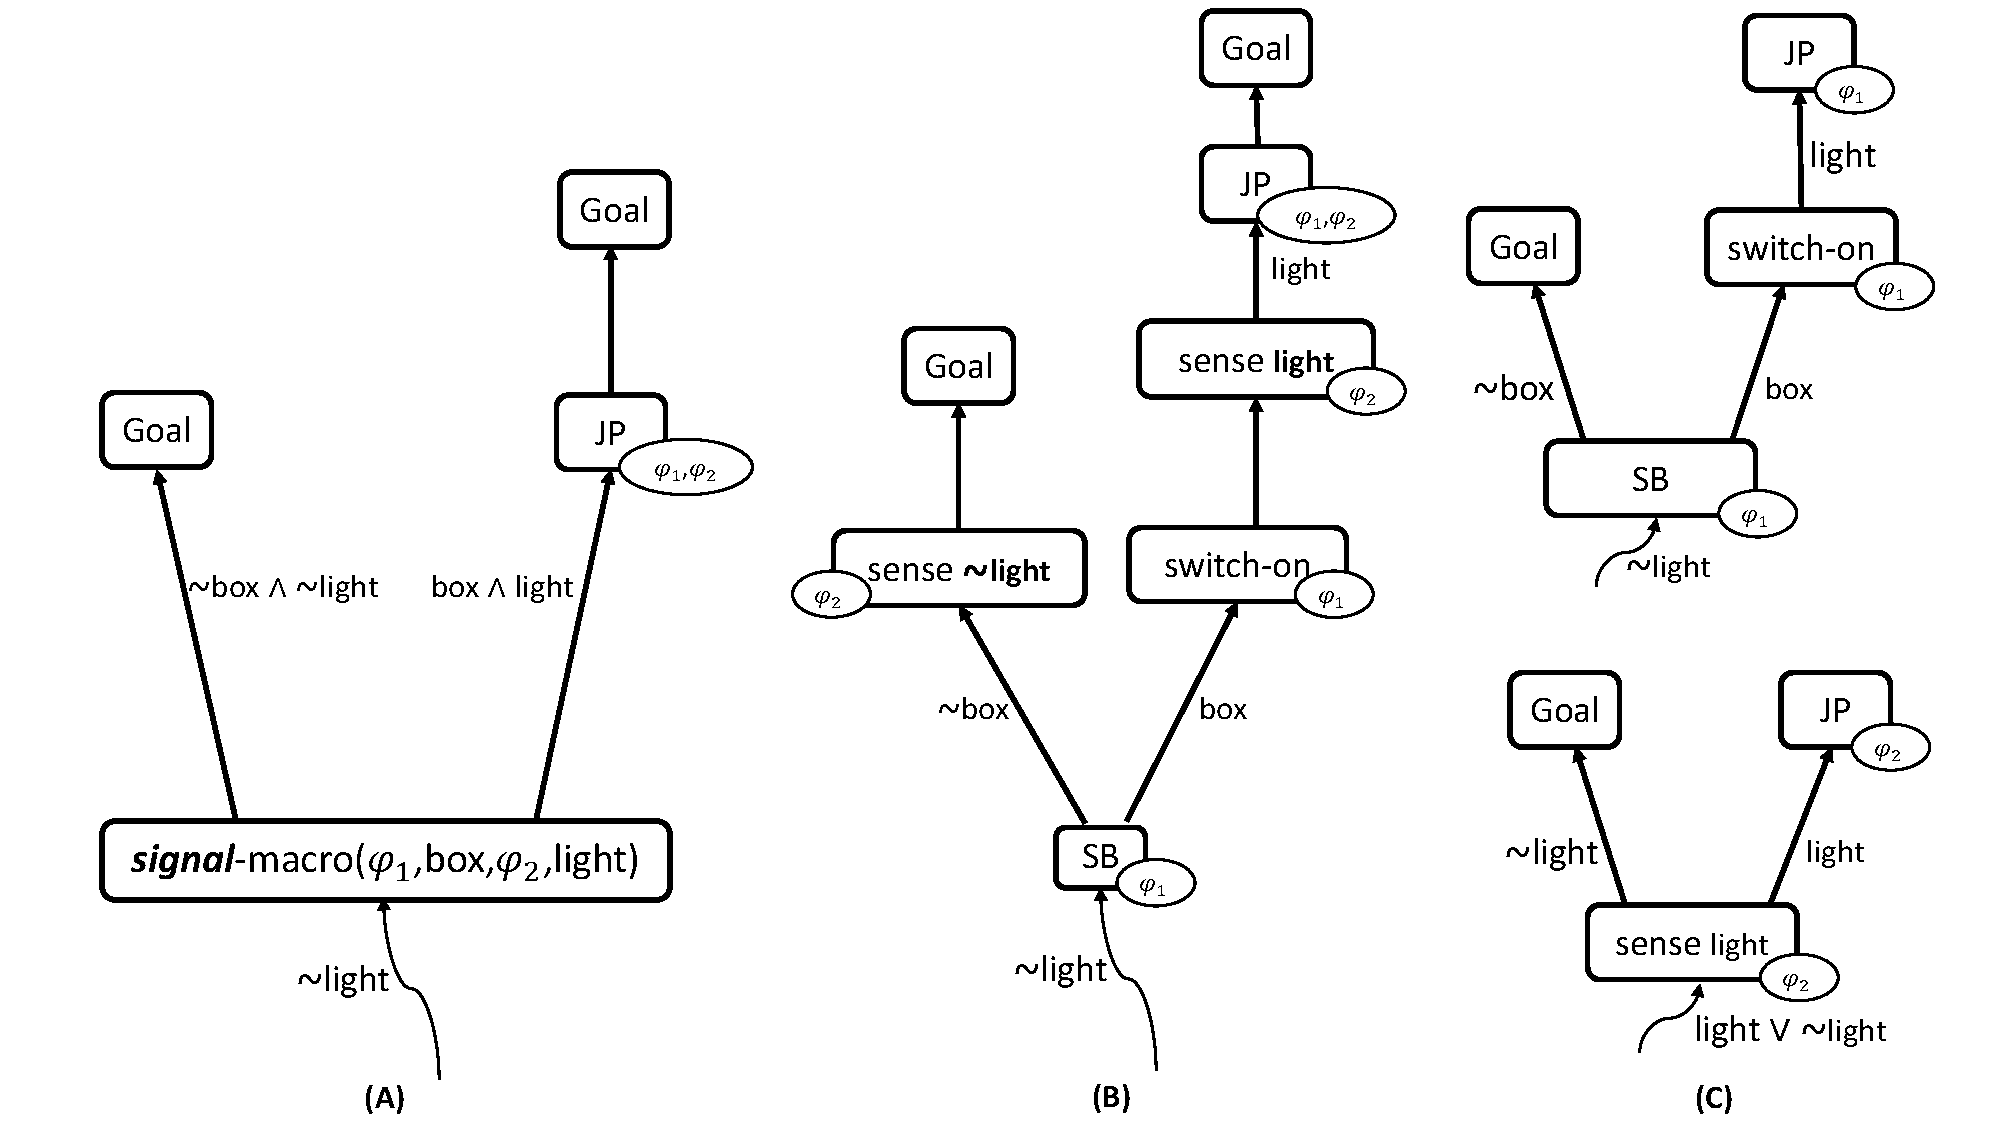
\includegraphics[height=2.6in, width=0.85\textwidth]{signaling-r.pdf}
\caption{
\emph{Signaling} in the QDec-FPS planner.
(A) A team plan with the signaling macro action.
(B) The team plan following the macro expansion.
(C) Projected trees for $\varphi_1$ (top) and $\varphi_2$ (bottom).
}
\label{fig:signaling}
\end{figure*}

\subsection{Signaling}
\label{subsec:signal}
If agent $\varphi_i$ can sense $p$ but agent $\varphi_j$ cannot, $\varphi_i$ might be able to communicate $p$'s value to $\varphi_j$.
It could do this directly, if an explicit communication action exists, or indirectly, by setting the value of some variable $q$ that agent $\varphi_j$ can sense, to be correlated with $p$'s value.
In fact, explicit communication can be viewed as correlating the value of a channel variable with $p$.
Signaling consists of the following steps (1) $\varphi_i$ senses $p$. (2) $\varphi_i$ sets the value of $q$ to the value of $p$. (3)  $\varphi_j$ senses $q$. (4) $\varphi_j$ reasons about the value of $p$.

Notice that (2) is not a restriction on a single branch of the plan, but a restriction on a sub-tree. $\varphi_i$ must ensure that $p\leftrightarrow q$, which means that it needs to act differently in the
branch where $p$ is true and in the branch where $p$ is false.

To operationalize this idea, we suggest to model the signaling process as a macro.
In our context, macros are not simply
a sequence of actions, but rather a sub-tree.

To construct such macros, we must first discover the possible signaling options. We preprocess the domain seeking quadruples $(\varphi_i, p, \varphi_j, q)$ such that
(1) $\varphi_i$ can sense $p$ but $\varphi_j$ cannot. (2) $\varphi_j$ can sense $q$.
(3) $\varphi_i$ can modify the value of $q$.
For simplicity, we consider only propositions $q$ that can be affected by a single action that does not change the value of any other public proposition. This can be extended to more complex sub-plans for modifying the value of $q$.
For each such quadruple, we add the macro-action $signal(\varphi_i, p, \varphi_j, q)$. Notice that this process is problem-instance {\em independent} and can be done in linear time.


The macro $signal(\varphi_i, p, \varphi_j, q)$ is treated by the planner as a sensing action that has two possible outcomes: in one of them $p\wedge q$ holds, and in the other $\neg p\wedge \neg q$ holds. Unlike the pure sensing actions we use, this action changes the state of the world, as well, ensuring that this correspondence between the values of $p$ and $q$ will hold.

Given a team plan with a signaling macro, we first expand the macro as indicated above: First, $\varphi_i$ senses the value of $p$. For each of the two resulting branches, it must ensure that $q$'s value is appropriately correlated, by applying actions that affect $q$'s value appropriately. Then, we add in each branch a sensing action $a_q$ where $\varphi_j$ senses the value $q$. While regular sensing actions have two possible children, $a_q$ has only a single child in the team plan because, at the team level, its outcome is known.
When projected to $\varphi_j$'s local plan, however, $a_q$ appears like a regular sensing action. This macro expansion is described in Figure~\ref{fig:signaling}.



In the next step, the projection of the team plan containing the macro expansion is solved by each agent. This requires, in particular, that agent $\varphi_i$ will change the value of $q$ as needed in each branch, and that both agents perform their sensing actions --- $\varphi_i$ over $p$ and $\varphi_j$ over $q$.

Figure~\ref{fig:signaling} shows an example of this process. Two agents, $\varphi_1$ and $\varphi_2$ must jointly push a heavy box. $\varphi_1$ can sense the box, but $\varphi_2$ can only sense whether a light is on. $\varphi_1$ can  signal to $\varphi_2$ about the box by turning on the light, which is originally off. Figure~\ref{fig:signaling}A shows a team plan with a macro.
Figure~\ref{fig:signaling}B shows the team plan after macro expansion: $\varphi_1$ senses the box, then turns on the light, if needed, and then $\varphi_2$ senses the light. Finally, both jointly push the box.
Figure~\ref{fig:signaling}C shows the projected single agent plan trees for $\varphi_1$ and $\varphi_2$.  %$\varphi_2$'s plan contains two children for the {\em sense-light} action, although the team plan does not. This special case is handled in the projection creation for which a time tick (T) is shown in the right (just for a reference).



In practice, adding this macro on top of an online contingent solver that focuses on a single branch at a time, such as SDR, is not straightforward. To address this, we do the following:
We add an action by $\varphi_i$ that can be viewed as a commitment to ensure that $p\leftrightarrow q$ holds. This action is constrained to be followed immediately by the action of sensing $p$ by $\varphi_i$.
At this point, in the team plan, if agent $\varphi_j$ needs to know the value of $p$, it can use the fact that $p\leftrightarrow q$ to deduce it from the value $q$. To ensure that it learns the value of $p$, we force the action of sensing $q$ in both branches.
As above, the team plan is post-processed to ensure that $\varphi_i$ does indeed ensure the validity of $p\leftrightarrow q$ following the sensing action.







\subsubsection{QDec-FPS Properties.}
When discussing soundness and completeness, we should first
distinguish between the abstract approach used by QDec-FP/S, which reduces multi-agent contingent planning to single-agent contingent planning, and the practical implementation of the planner which uses a specific planner, CPOR.

First, consider the abstract formulation and assume a sound and complete underlying single-agent contingent planner. The soundness of QDec-FPS without signaling follows from that of QDec-FP: Every team solution of QDec-FPS is also a possible team-solution for QDec-FP and all the other steps are identical. This remains true in the implementation due to the soundness of CPOR.

With signaling, the abstract version of the macro is a sensing action with effects.
It remains sound if the action used by the signaling agent to ensure that $p\leftrightarrow q$ holds does not affect any other proposition. The implementation using CPOR is more complex, but it ensures that following the commitment to the signaling macro, the team solution implements a correct version of the macro, and hence it is sound, too.

In the case of completeness, for QDec-FPS, one cannot
separate between an abstract and implemented case because the core contribution of QDec-FPS is at the level of
the implementation of the classical encoding used by CPOR and SDR. At this level, QDec-FPS is incomplete for two
reasons: First, CPOR is an incomplete solver: it lacks an internal backtracking mechanism. (For that reason, the implementation of QDec-FP is also incomplete, although the abstract formulation is complete.)
Second, the planner's ability to reason about the knowledge of separate agents, as implemented at present, is incomplete. That is, it can under-estimate the knowledge of an agent. Thus, it might not be able to deduce that the preconditions of some actions are known to the acting agent, even though they are.





































\begin{table}[ht!]
\centering
\resizebox{\columnwidth}{!}{%
\begin{tabular}{@{}l | l | r | r@{}r | r r | r r | r r@{} }
\hline \cline{1-11}
\multicolumn{1}{@{}l|}{\multirow{2}{*}{\textbf{Domain}}} & \multicolumn{1}{c|}{\multirow{2}{*}{\textbf{Ins (\#agt)}}} & \multicolumn{1}{c|}{\multirow{2}{*}{\textbf{Objects}}} & \multicolumn{2}{c}{\multirow{1}{*}{\textbf{Max-width} }}
& \multicolumn{2}{c}{\multirow{1}{*}{\textbf{Max-height} }}
& \multicolumn{2}{c}{\multirow{1}{*}{\textbf{Time (sec)} }}
& \multicolumn{2}{c}{\multirow{1}{*}{\textbf{BT} }}\\
\cline{4-11}
& & & \emph{fp} & \emph{fps} & \emph{fp} & \emph{fps} & \emph{fp} & \emph{fps} & \emph{fp} & \emph{fps} \\
\hline \cline{1-11}
\multicolumn{1}{@{}l|}{\multirow{16}{*}{\textbf{BP}}}
& B1 (3) &16	&8		&5	&23	&18	&3.59		&\textbf{2.91} 	&0		&0 \\
& B2 (4) &16	&12		&10	&19	&19	&\textbf{5.3}		&6.1 	&0		&0 \\

& B3 (9) & 36	& 64 & *	& 24	& *	& \textbf{25.3}	& *	& 0 & * \\
\cdashline{2-11} %\cdashline{2-11}
& B4 (3) & 11	& 4	& 4	& 14	& 11	& 16.39	& \textbf{1.17}	& 9	& 0 \\

& B5 (3) & 12	& 6	& 8	& 16	& 15	& 13.65	& \textbf{2.9}	& 4	& 0 \\ 						& B6 (3) & 12	& -		& 6	&	- 	& 12	& - 		& \textbf{13.58}	& {47}$^{\tiny +}$ 	& 4 \\
& B7 (3) & 12	& 8	& 8	& 18	& 19	& 158.89 & 	\textbf{3.87}	& 41	& 0 \\
& B8 (3) & 12	& 8	& 8	& 17	& 21	& 111.6	& \textbf{4.05}	& 26	& 0 \\
& B9 (3) & 13	& 16	& 14	& 21	& 19	& 121.42 & 	\textbf{5.6}	& 19	& 0 \\
& B10 (3) & 16	& 16	& 15	& 26	& 29	& 155.83 & 	\textbf{9.69}	& 33	& 0 \\
& B11 (5) & 20	& * & 24	& *	& 32	& *	& \textbf{75.21}	& *	& 1 \\
& B12 (5) & 20	& * & 24	& *	& 37	& *	& \textbf{365.9}	& *	& 6 \\
\cdashline{2-11} %\cdashline{2-11}
& B13 (2) & 10	& \emph{na}	& 2	& \emph{na}	& 6	& \emph{na}	& \textbf{1.06}	& \emph{na}	& 0
\\

& B14 (2) & 12	& \emph{na}	& 2	& \emph{na}	& 2	& \emph{na}	& \textbf{1.20}	& \emph{na}	& 1 \\

& B15 (3) & 12	& \emph{na}	& 4	& \emph{na}	& 12	& \emph{na}	& \textbf{2.49}	& \emph{na}	& 0 \\						& B16 (3) & 13	& \emph{na}	& 4	& \emph{na}	& 7	& \emph{na}	& \textbf{5.5}	& \emph{na}	& 1 \\
& B17 (3) & 13	& \emph{na}	& 4	& \emph{na}	& 6	& \emph{na}	& \textbf{8.9}	& \emph{na}	& 2 \\

& B18 (3) & 14	& \emph{na}	& 6	& \emph{na}	& 16	& \emph{na}	& \textbf{4.04}	& \emph{na}	& 0 \\

& B19 (4) & 15	& \emph{na}	& 8	& \emph{na}	& 14	& \emph{na}	& \textbf{17.6}	& \emph{na}	& 2 \\

\hline \cline{1-11}
\multicolumn{1}{@{}l|}{\multirow{15}{*}{\textbf{TM}}}
& T1 (3) & 10 	&8	&7	&20	&16	&\textbf{2.68}	&2.78	&0	&0  \\
& T2 (4) & 12 	&16	&13	&21	&17	&\textbf{7.84}	&8.26 &0 &0  \\
& T3 (4) & 15 	&12	&16	&34	&26	&\textbf{8.74}	&12.39		&0	&0  \\
& T4 (5) & 14 	&19	&22	&22	&24	&\textbf{20.5} &43.58	&0	&0 \\ %removedVspace

& T5 (5) & 16	&12	&14	&32	&25	&\textbf{9.7}		&11.2	&0	&0 \\
\cdashline{2-11}
& T6 (3) & 8	& 2	& 2	&8	&8	& 11.01 	& \textbf{0.61}	& 7	& 0 \\
& T7 (3) & 10 	&8	&7	&20	&16	&\textbf{34.5}	&41.8	&8	&8  \\
& T8 (3) & 10 	&8	&8	&24	&22	&37.87	&\textbf{22.45}	&9	&4  \\
& T9 (3) & 10 	&-	&-	&-	&-	&140.32	&\textbf{29.73}		&31	&6  \\
& T10 (4) & 12 	&16	&16	&23	&22	&\textbf{6.68}	&152.18	&0	&14  \\
& T11 (5) & 16	&16	&16	&30	&35	&274.5		&\textbf{56.15}		&27	&3 \\
\cdashline{2-11}
& T12 (2) & 10	& \emph{na}	& 2		& \emph{na}	& 9		& \emph{na}	& \textbf{1.7}	& \emph{na}	& 0 \\
& T13 (2) & 12 	&\emph{na}	&4		&\emph{na}	&17	& \emph{na}	& \textbf{6.81}	& \emph{na}		&0 \\
& T14 (3) & 12 	&2		&2		&16	&11	& 17.59	& \textbf{2.32}	& 9		&0 \\
& T15 (3) & 13 	&\emph{na}	&4		&\emph{na}	&14	& \emph{na}	& \textbf{7.80}	& \emph{na}		&0 \\
& T16 (3) & 14  	&\emph{na}	&4		&\emph{na}	&19	& \emph{na}	& \textbf{11.68}	& \emph{na}		&1 \\
\hline
\cline{1-11}
\multicolumn{1}{c|}{\multirow{22}{*}{\textbf{\textcolor{black}{Rovers}}}}
& R1 (1) & 12 & 2 & 2	&8	&8	& 3.8 & 3.8 & 0	& 0 \\
& R2 (2) & 14 & 2 & 2	& 9	& 8	& 5.4 	& \textbf{5.3}	& 0	& 0 \\

& R3 (2) & 13 & 4 & 4	& 15	& 15	& 9.3 	& \textbf{8.9}	& 0	& 0
\\
& R4 (2) & 17   & 12  & 12	& 34	& 23	& \textbf{35.8} 	& 38.6	& 0	& 0
\\
& R5 (3) & 18	&12	&12	&28	&32	&\textbf{51.5}	&54.1	&0	&0
\\
& R6 (3) & 21	&30	&30	&36	&29	&136.6	&\textbf{111.9}	&0	&0
\\
& R7 (3) & 23	&98	&81	&50	&45	&567.9	&\textbf{233.2}	&0	&0
\\
\cdashline{2-11}
& R8 (3) &13    &2	&2	&7	&6	&57.9	&\textbf{5.9}   &3	&0
\\
& R9 (3) &14	&4	&4	&12	&12	&113.8	&\textbf{10.2}	&4	&0
\\
& R10 (3) &14	&4	&4	&11	&11	&314.5	&\textbf{89.3}	&11	&3
\\
& R11 (3) &19	&-	&12	&-	&12	&325.1	&\textbf{41.1}	&6+	&0
\\
& R12 (4) &15	&4	&4	&12	&11	&47.2	&\textbf{16.0}	&1	&0
\\
& R13 (4) &20	&12	&12	&25	&19	&241.8	&\textbf{49.1}	&3	&0
\\
\cdashline{2-11}
& R14 (2) &16	& \emph{na}	& 2	&\emph{na}	&9	&\emph{na}	&\textbf{3.6}	&\emph{na}	&0
\\
& R15 (2) & 18	& \emph{na}	& 2	&\emph{na}	&10	&\emph{na}	&\textbf{5.89}	&\emph{na}	&0
\\
& R16 (2) & 16	& \emph{na}	& 4	&\emph{na}	&13	&\emph{na}	& \textbf{34.17}	&\emph{na}	&0
\\
& R17 (2) & 20	& \emph{na}	& 4	&\emph{na}	& 14	&\emph{na}	& \textbf{17.68}	&\emph{na}	&0
\\
& R18 (3) & 17	& \emph{na}	& 2	&\emph{na}	&7	&\emph{na}	& \textbf{10.17}	&\emph{na}	&0
\\
& R19 (3) & 18	& \emph{na}	& 4	&\emph{na}	&13	&\emph{na}	& \textbf{12.93}	&\emph{na}	&0
\\
& R19 (3) & 14	& \emph{na}	& 2	&\emph{na}	& 7	&\emph{na}	& \textbf{6.62}	&\emph{na}	&0
\\
& R20 (3) & 19	& \emph{na}	& 8	&\emph{na}	&16	&\emph{na}	& \textbf{36.74}	&\emph{na}	&0
\\
& R21 (4) & 20	& \emph{na}	& 6	&\emph{na}	&11	&\emph{na}	& \textbf{67.79}	&\emph{na}	&0
\\
& R22 (4) & 22	& \emph{na}	& 6	&\emph{na}	&12	&\emph{na}	& \textbf{68.21}	&\emph{na}	&0
\\
\hline
\end{tabular}
}
\caption{
Comparison of QDec-FP and QDec-FPS planners.
\emph{Ins (\#agt)}: instance number and
number of acting agents.
\emph{Object}: the number of objects in each problem.
\emph{BT}: number of planner backtracks.
\textbf{*}: time out. '\textit{-}':  planner could not solve or breaks down.  \emph{na}: problem not applicable to a solver. \emph{fp}: QDec-FP.
\emph{fps}: QDec-FPS. The best approach, based on time only, is shown in bold.
}
\label{tbl:final-results}
\end{table}



\section{Empirical Evaluation}

We now examine the applicability and scalability of QDec-FPS by comparing it with QDec-FP on 3 multi-agent planning domains.
Some problems in each domain were modified to require \emph{signaling}.
Both QDec-FP and QDec-FPS are  implemented in C\#, and were run on a Windows 10, 64 bit machine with \emph{i}7 processor, 2.8GHz CPU, and 16Gb RAM.
IMAP was not considered, as QDec-FP was  shown to scale better than IMAP~\citep{IMAP}.

We experiment with the following three domains:

\noindent{\bf Box-Pushing (BP)}: Boxes located in a grid-like structure. Each box is to be pushed to its destination location
outside the column the box appears in \citep{BrafmanSZ13}.
A light box can be pushed by a single agent co-located with the box while a heavy box requires two co-located agents.
Agents can be non-homogeneous, i.e., different agents can observe and push different boxes.

\noindent{\bf Table-Mover (TM)}: TM consists of a number of tables and rooms, and agents that can move between connected rooms \citep{ShekharB20}.
The tables' locations are uncertain initially, and agents must move them to their goal locations.
Agents can be non-homogeneous in their sensing and manipulation abilities.
All table manipulation actions are collaborative:
\emph{2move-table}, \emph{2lift-table}, \emph{2drop-table}.

\noindent{\bf Rovers}:
Multiple rovers navigate a planet surface, finding samples and communicating them back to a lander \citep{IMAP}.
Two rovers must simultaneously collect the rock sample, while a single agent can sample soil as well as take images of certain objectives on its own.
Coordination points include locations (waypoints) which are accessible to multiple rovers. Rovers communicate sampled soil/image/rock data to the lander that exists at a certain waypoint.
A rover navigates between two waypoints
and must be present at the corresponding %waypoint
to sample.
Availability of data to sample at a waypoint is unknown to the rovers initially.
In this modified domain, our schema requires two rovers working jointly to collect rock samples. After taking measurements, the rovers must broadcast them back to the lander.
In this domain in general, a rover has fewer public actions (approx. 46\% on average), but a relatively complex internal planning problem, including navigation, soil and rock sampling, and image capturing.

Table~1 compares QDec-FPS and QDec-FP based on policy quality (\emph{max-width}, \emph{max-height}), runtime (\emph{time}), and the number of \emph{backtracks}  required.
\emph{max-width} and \emph{max-height} refer to maximum number of branches and the maximum height of all individual solution trees obtained for the agents.
The number of branches is also indicative of the number of sensing actions performed, as branching occurs following an observation.
The planner backtracks when at least one of the single-agent problems, obtained by decomposing $\tau_{team}$, is unsolved by CPOR.
Within each domain in the table, dashed lines separate three problem classes: homogeneous agents,
non-homogeneous agents, and non-homogeneous agents that require signaling.  To handle signaling, QDec-FPS adds macros, which may have a significant overhead. Therefore, these macros were only added in problems that require signaling. The decision whether to add macros was done {\em manually}. In the future, we will automatically detect whether signaling is needed.


In BP, QDec-FPS scales much better than QDec-FP in problems with three  to five agents. Increasing the number of objects had minor impact on QDec-FPS running time, as opposed to QDec-FP. For many problems, QDec-FPS needs to backtrack fewer times than QDec-FP, and as a result, it finds solutions faster.
On the other hand, increasing the number of agents has an adverse effect on  QDec-FPS.
In fact, instance B3 in the BP domain with nine {\em identical} agents, was quite rapidly solved by QDec-FP, while QDec-FPS times out.
This is because the new translation makes the team problem much harder to solve. Thus, QDec-FP finds a team plan quickly,
and when agents are identical, it is usually very easy to fix the team problem by adding any needed sensing action. For that reason, in the case of homogenous agents, we see no
backtracks in any of the problems.
On the other hand, problems B11 and B12 were solved by the QDec-FPS planner but were unsolved by QDec-FP. This is most likely due to the high number of required backtracks. We can conclude that for simpler problems with identical agents, QDec-FP scales better with the number of agents, but for more complex problems, QDec-FPS is required.  Unlike BP, in  TM each public action is a collaborative action.
Similar to the BP domain, when backtracking is not required to solve an instance, for example, the simpler instances T1 to T5, the QDec-FP solver takes less time to solve it than that of QDec-FPS.
When problems are more complex and backtracking is required, e.g., for the instances T6 and T11, QDec-FPS is faster.  In Rovers, we see a similar trend as BP and TM.
For the simple instances like R1 to R7, the performance of the planners is mixed.
When backtracking maybe required since the rovers are non-homogeneous (instances R8 to R13), QDec-FPS outperforms QDec-FP on all instances. Instances with more objects are solved relatively easily by QDec-FPS.














Problem T9 is interesting because it is unsolvable.
This requires the planner to rule out all possible solutions. Because the team problem QDec-FPS generates has fewer solutions, it was able to
rule them out much faster
using six backtracks, compared to 31 for QDec-FP.

The table clearly shows that QDec-FPS generates smaller trees across all domains. A closer inspection of the policies also shows that the number of {\em noops} in its solution is smaller.

To test signaling, we added new instances to all domains that cannot be solved without signaling (B13-B19, T12-T16, R14-R22). These instances cannot be solved
by QDec-FP (shown as \emph{na}).
In the BP instances, moving from 2-3 agents to 4 increased runtime by an order of magnitude. This is likely due to the number of optional pairwise signaling added with each agent. However, adding objects did not much impact runtime.
In the TM domain, we see a more mixed picture. Adding agents or objects can increase run-time, although not always (e.g. T14 vs. T12 and T13).
T14 is particularly interesting because it can be solved without signaling (hence QDec-FP solves it with 9 backtracks), but it is solved even faster with signaling.
For this instance there are three agents, $\varphi_1$, $\varphi_2$, and $\varphi_3$ such that $\varphi_1$ and $\varphi_3$ together are capable of solving this problem without signaling.
As we purposely placed $\varphi_3$ farther from the table's location, QDec-FPS generated a plan where $\varphi_1$ signaled to $\varphi_2$ the table's location and they achieved the goal together, without $\varphi_3$. This solution was generated much quicker and with no backtracks.
Signaling in Rovers is similar to BP.
Adding more agents makes the problem harder,
especially when we move to 4 agents, whereas the effect of objects is less clear.
The number of instances of signaling macros in the team solutions range from 1 to 4 on larger problem instances.

\section{Conclusion}

QDec-FPS uses a
factored approach that solves a MAP problem
by reducing it to multiple single-agent planning problems. By
reasoning about individual agents' knowledge, it generates more informed team plans that
lead to fewer backtracks and better scalability. This ability
allows it to also
support signaling, a form of
implicit communication
through the state of the world,
and thereby to solve
problems unsolvable by previous planners.

\noindent{\bf Acknowledgements.}  This work was supported by ISF Grants 1651/19 and 1210/18, by the Israel Ministry of Science and Technology Grant 54178, and by the Lynn and William Frankel Center for Computer Science.
\bibliographystyle{aaai}
Quod nisi nihil ipsam, vero accusamus doloribus ab quia, tempora velit tempore iste quae voluptatum possimus, voluptates perferendis sed nulla aliquid a dignissimos saepe blanditiis, cumque architecto molestiae tenetur omnis totam laborum impedit eum itaque ipsa?Rem incidunt minima provident explicabo magni eius saepe rerum aspernatur dolore, fugit dolorum amet architecto, quo velit similique culpa molestiae, rem eveniet saepe vero sapiente laboriosam quos illo id, veniam tempore deserunt in alias.\clearpage
\bibliography{icaps20-ws.bib}

\end{document}


